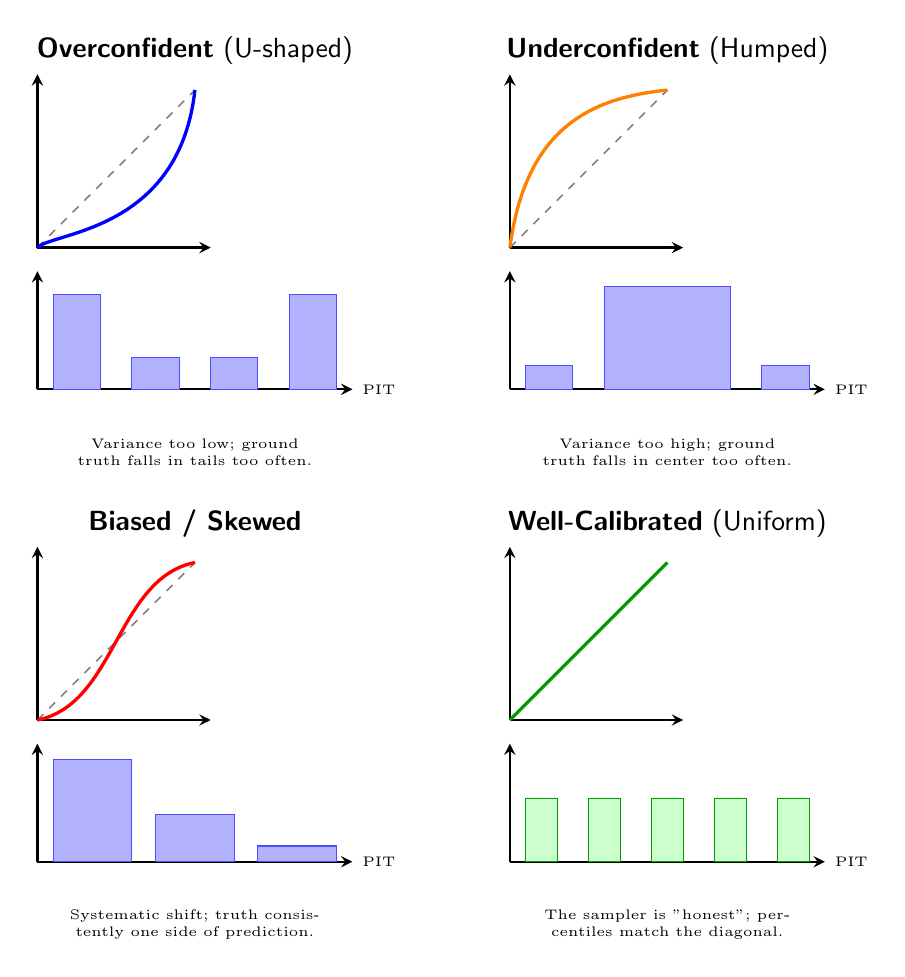
\begin{tikzpicture}[font=\sffamily]

% --- Define Styles ---
\tikzset{
    axis/.style={->, >=stealth, line width=0.8pt},
    diag/.style={dashed, gray, line width=0.6pt},
    pitbar/.style={fill=blue!30, draw=blue!70},
    cdfline/.style={line width=1.2pt},
    box/.style={draw=gray!30, rounded corners=5pt, inner sep=10pt}
}

% ================= 1. OVERCONFIDENT =================
\begin{scope}[shift={(0,0)}]
    \node[anchor=south] at (2,4) {\textbf{Overconfident} (U-shaped)};
    % Histogram
    \draw[axis] (0,0) -- (4,0) node[right, font=\tiny] {PIT};
    \draw[axis] (0,0) -- (0,1.5);
    \draw[pitbar] (0.2,0) rectangle (0.8,1.2);
    \draw[pitbar] (1.2,0) rectangle (1.8,0.4);
    \draw[pitbar] (2.2,0) rectangle (2.8,0.4);
    \draw[pitbar] (3.2,0) rectangle (3.8,1.2);
    
    % CDF Plot
    \begin{scope}[shift={(0,1.8)}]
        \draw[diag] (0,0) -- (2,2);
        \draw[axis] (0,0) -- (2.2,0);
        \draw[axis] (0,0) -- (0,2.2);
        % Sigmoid-ish curve crossing diagonal
        \draw[cdfline, blue] (0,0) .. controls (0.2,0.2) and (1.8,0.2) .. (2,2);
    \end{scope}
    \node[text width=4cm, align=center, font=\tiny] at (2,-0.8) {Variance too low; ground truth falls in tails too often.};
\end{scope}

% ================= 2. UNDERCONFIDENT =================
\begin{scope}[shift={(6,0)}]
    \node[anchor=south] at (2,4) {\textbf{Underconfident} (Humped)};
    % Histogram
    \draw[axis] (0,0) -- (4,0) node[right, font=\tiny] {PIT};
    \draw[axis] (0,0) -- (0,1.5);
    \draw[pitbar] (0.2,0) rectangle (0.8,0.3);
    \draw[pitbar] (1.2,0) rectangle (2.8,1.3);
    \draw[pitbar] (3.2,0) rectangle (3.8,0.3);
    
    
    % CDF Plot
    \begin{scope}[shift={(0,1.8)}]
        \draw[diag] (0,0) -- (2,2);
        \draw[axis] (0,0) -- (2.2,0);
        \draw[axis] (0,0) -- (0,2.2);
        % Inverse Sigmoid
        
        \draw[cdfline, orange] (0,0) .. controls (0.2,1.5) and (1,1.9) .. (2,2);
    \end{scope}
    \node[text width=4cm, align=center, font=\tiny] at (2,-0.8) {Variance too high; ground truth falls in center too often.};
\end{scope}

% ================= 3. BIASED / SKEWED =================
\begin{scope}[shift={(0,-6)}]
    \node[anchor=south] at (2,4) {\textbf{Biased / Skewed}};
    % Histogram
    \draw[axis] (0,0) -- (4,0) node[right, font=\tiny] {PIT};
    \draw[axis] (0,0) -- (0,1.5);
    \draw[pitbar] (0.2,0) rectangle (1.2,1.3);
    \draw[pitbar] (1.5,0) rectangle (2.5,0.6);
    \draw[pitbar] (2.8,0) rectangle (3.8,0.2);
    
    % CDF Plot
    \begin{scope}[shift={(0,1.8)}]
        \draw[diag] (0,0) -- (2,2);
        \draw[axis] (0,0) -- (2.2,0);
        \draw[axis] (0,0) -- (0,2.2);
        % Concave curve
        \draw[cdfline, red] (0,0) .. controls (1,0.2) and (1,1.8) .. (2,2);
    \end{scope}
    \node[text width=4cm, align=center, font=\tiny] at (2,-0.8) {Systematic shift; truth consistently one side of prediction.};
\end{scope}

% ================= 4. WELL-CALIBRATED =================
\begin{scope}[shift={(6,-6)}]
    \node[anchor=south] at (2,4) {\textbf{Well-Calibrated} (Uniform)};
    % Histogram
    \draw[axis] (0,0) -- (4,0) node[right, font=\tiny] {PIT};
    \draw[axis] (0,0) -- (0,1.5);
    \foreach \x in {0.2, 1, 1.8, 2.6, 3.4}
        \draw[pitbar, fill=green!20, draw=green!60!black] (\x,0) rectangle (\x+0.4, 0.8);
    
    % CDF Plot
    \begin{scope}[shift={(0,1.8)}]
        \draw[diag] (0,0) -- (2,2);
        \draw[axis] (0,0) -- (2.2,0);
        \draw[axis] (0,0) -- (0,2.2);
        % Perfectly on diagonal
        \draw[cdfline, green!60!black] (0,0) -- (2,2);
    \end{scope}
    \node[text width=4cm, align=center, font=\tiny] at (2,-0.8) {The sampler is "honest"; percentiles match the diagonal.};
\end{scope}

\end{tikzpicture}